\documentclass{article}
\usepackage[utf8]{inputenc}
\title{Comp110 research journal}
\author{PH230156}

\usepackage{natbib}
\usepackage{graphicx}
\graphicspath{ {./images} }
\setlength{\parskip}{1em}
\begin{document}

\maketitle

\section{Journal entry No.1 in Alpha-Beta Pruning:}

\underline Comp110 – Research journal
\par An analysis of alpha-beta pruning[1]
\par \underline Section 1a – The concept behind alpha-beta analysis:
Alpha-beta analysis is a way of looking at how to carry out tasks, generate ideas and so on. When alpha-beta is used in games, in either playing it or developing games, it can be used effectively to deliver good game mechanics, such as chess where each turn can affect the game in more ways the longer the game is played, or in developing games, it can branch into more things to add into the development of a game, such as a main story can introduce side quest characters by adding them into the main story as a vital key to progressing in a game.

\par
•	1: Alpha-beta pruning is a search algorithm that computers can use to cut the time in searching for items in a big list. The computer checks the first character of the specified word that a user has desired, and finds where the first letter is in the list, as an example “Verge” is the specified word. The program checks the first half of the list (A-M or N) for the first letter (V), and can’t find it, so it cuts off it’s search range in half. The computer keeps reducing it’s search range in half until it finds the specified word.
\par
\underline Section 1b – A real look at alpha-beta pruning:
To really see what alpha-beta pruning is, you need to look at a process tree. As an example, we will talk about the game Chess, and how a computer plays chess. The computer has what is called a process tree, and with this tree, it can determine what moves the player is going to make, for example the player can move one of 2 knights in 4 different places, or move one pawn forwards twice, or once. The longer the game is played, the more processes that could occur are shown in the tree, The computer will keep going down the process tree until the game has ended, either victory, draw or defeat. The way that chess computers use alpha-beta pruning, is by exploring each move it can make and deciding which option will be the most beneficial to allow the computer to win.
An image is shown below to provide more illustration to my definition:

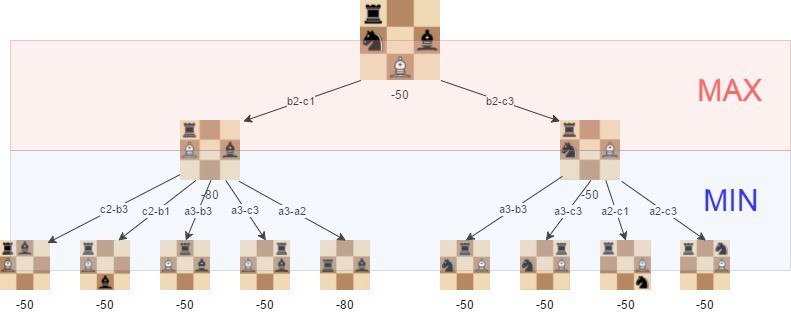
\includegraphics[scale=0.5]{alpha-beta.jpeg}
image source: \textit{https://cdn-media-1.freecodecamp.org/images/1*UA5VlNs7s4gl80VknA099w.jpeg}

\par Source of image: \textit{https://www.freecodecamp.org/news/simple-chess-ai-step-by-step-1d55a9266977/}


\underline{Section 2a – Complex games with alpha-beta pruning:}

Complex games most of the time prevent computers from search all possible outcomes in a process tree, even in chess sometimes the game becomes too complicated for the computer to be accurate. This can be fixed if the algorithm has a intentional function of pretending that after so many moves, there are no successful moves that each player can make, this cuts the amount of processing the computer does in order to be accurate in its moves. Even allowing the computer to only process one branch will remove the complexity of a process tree, for example if the player moves the knight twice in a row, the computer can remove all the other possible branches that are not connected to the initial branch.

\underline{Section 2b – History of alpha-beta pruning:}
The origin of alpha-beta pruning was located in Russia, in a Russian chess-playing program, where Alexander Brudno described this algorithm which is similar to alpha-beta pruning, in 1963. The finalised version of alpha-beta pruning appeared in the Western computer literature in 1958 in an article on strategies. This took many years to properly publish since it was so misunderstood, you had to be very good at mathematics to actually understand the concept; although now we have algorithmic languages at our disposal, it can easily be understood through the use of pseudocode and illustration of functions.

\par
\underline Section 3a – Do we need to look at the whole process tree?:
As it turns out, no. Computers do not have to look at every possible outcome on every branch, this would take a considerable large amount of unnecessary computation to do nothing as you’ll see in a bit. As I said earlier, the computer doesn’t need to look at every branch, this means that the nodes it doesn’t need to look at can pretend like they never existed, this is because those nodes won’t be able to affect a better outcome overall, for example, in a game of chess, there is a process tree, at the top of the process tree there is no value, but has two variables, one called Min and one called Max, the program calls to each tree on its left (depending on how many turns in the future it goes to), it finds the highest value and then stores it in the node above where it found the value. Then it calls to the other branch on the same level as the value, if the second value is higher than the first value, it is put into the node above the values instead of the first one. Then, the 2 values are checked against each other, and picks the smallest one, this is Min’s turn (Min is making sure to keep the numbers as low as possible to stop the player from succeeding as much). Min and Max are being used by the program to allow the computer to benefit more than the player.

\bibliographystyle{plain}
\bibliography{references}

\cite{knuth1975_alphabeta}
\cite{Simple_chess_AI}
\cite{Alpha_beta_pruning}


\end{document}
